\documentclass[]{standalone}
%\usepackage{mathptmx}
%\renewcommand{\familydefault}{\rmdefault}
\usepackage[T1]{fontenc}
\usepackage[latin9]{inputenc}
\usepackage{siunitx}
\usepackage{array}
\usepackage{amsmath}
\usepackage{ifthen}
\usepackage{pgfplots}
\pgfplotsset{compat=1.14}
\usepackage{titling, graphicx}
\usepackage{tikz}
\usepackage{upgreek}
\usepackage{amsmath,amsthm}
\usepackage{strtikz}
\usetikzlibrary{shapes,arrows.meta,intersections,graphs,graphs.standard}
\usetikzlibrary{math,fit}
\usetikzlibrary{calc,intersections,through,backgrounds,decorations.pathmorphing}


\begin{document}
\begin{tikzpicture}
\framerigid[startx = 0cm,
starty = 0cm,
endx = 3cm,
endy = 5cm,
rigid start x = 1cm,
rigid start y = 2cm,
rigid end x= 1cm,
rigid end y= 2cm,
tick length = 0.4cm,
tick width = 0.5pt,
rigid end thickness = 3pt,
frame thickness = 1pt,
rigid color=blue,
frame color=black,
frame text node i = {$i'$},
frame text node j = {$j'$},
frame text = {$L, E, I, A$},
rigid text node i x = {$r_i^x$},
rigid text node i y = {$r_i^y$},
rigid text node i end = {$i$},
rigid text node j x = {$r_j^x$},
rigid text node j y = {$r_j^y$},
rigid text node j end = {$j$},
horizontal=6,]
\end{tikzpicture}
\end{document}